\documentclass{standalone}


\usepackage{tikz}
\usepackage{pgfplots}
\usetikzlibrary{calc}
\pgfplotsset{compat=1.15}
\usetikzlibrary{shapes,arrows.meta}
\begin{document}


% The block diagram code is probably more verbose than necessary
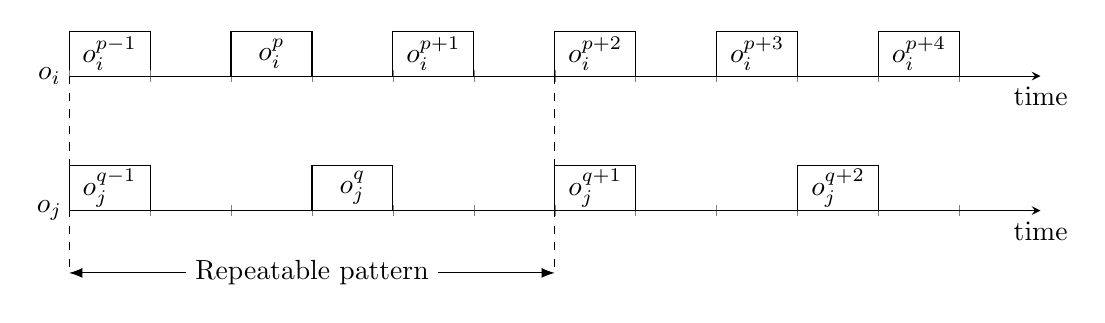
\begin{tikzpicture}[>=Latex]


\begin{axis}[
    xmin=0, xmax=6,
    axis x line=bottom,% only show the bottom x axis
    hide y axis,    
    ymin=0,ymax=2,
				xtick={0,0.5,1,1.5,2,2.5,3,3.5,4,4.5,5,5.5},
				xticklabels={,,},
				x label style={align=center,at={(current axis.right of origin)},anchor=east, above=-5mm},
				xlabel={time
				},
				x post scale=1.8
    ]
\addplot+[mark=none,const plot,draw=black]
coordinates
{(0,0) (0,0.2) (0.5,0.2) (0.5,0)};
\addplot+[mark=none,const plot,draw=black]
coordinates
{(1.5,0) (1.5,0.2) (2,0.2) (2,0)};
\addplot+[mark=none,const plot,draw=black]
coordinates
{(3,0) (3,0.2) (3.5,0.2) (3.5,0)};
\addplot+[mark=none,const plot,draw=black]
coordinates
{(4.5,0) (4.5,0.2) (5,0.2) (5,0)};


\addplot+[const plot,mark=none,draw=black]
coordinates
{(0,0.6) (0,0.8) (0.5,0.8) (0.5,0.6)};

\coordinate (s) at (axis cs:0,0.6);
\coordinate (u) at (axis cs:3,0.6);

\node at (axis cs:.25,0.1) {$o_j^{q-1}$};
\node at (axis cs:1.75,0.1) {$o_j^q$};
\node at (axis cs:3.25,0.1) {$o_j^{q+1}$};
\node at (axis cs:4.75,0.1) {$o_j^{q+2}$};
		
\end{axis}

\begin{axis}[at={(s)},
    xmin=0, xmax=6,
    axis x line=bottom,% only show the bottom x axis
    hide y axis,    
    ymin=0,ymax=2,
				xtick={0,0.5,1,1.5,2,2.5,3,3.5,4,4.5,5,5.5},
				xticklabels={,,},
				x label style={align=center,at={(current axis.right of origin)},anchor=east, above=-5mm},
				xlabel={time},
				x post scale=1.8
    ]

\addplot+[mark=none,const plot,draw=black]
coordinates
{(4,0) (4,0.2) (4.5,0.2) (4.5,0)};
\addplot+[mark=none,const plot,draw=black]
coordinates
{(5,0) (5,0.2) (5.5,0.2) (5.5,0)};
\addplot+[mark=none,const plot,draw=black]
coordinates
{(1,0) (1,0.2) (1.5,0.2) (1.5,0)};
\addplot+[mark=none,const plot,draw=black]
coordinates
{(2,0) (2,0.2) (2.5,0.2) (2.5,0)};
\addplot+[mark=none,const plot,draw=black]
coordinates
{(3,0) (3,0.2) (3.5,0.2) (3.5,0)};

\draw [dashed] (0,0) -- (0,-1);

\node at (axis cs:.25,0.1) {$o_i^{p-1}$};
\node at (axis cs:1.25,0.1) {$o_i^p$};
\node at (axis cs:2.25,0.1) {$o_i^{p+1}$};
\node at (axis cs:3.25,0.1) {$o_i^{p+2}$};
\node at (axis cs:4.25,0.1) {$o_i^{p+3}$};
\node at (axis cs:5.25,0.1) {$o_i^{p+4}$};


\end{axis}

\node [xshift=-.25cm] at (0,0) {$o_j$};
\node [xshift=-.25cm] at (s) {$o_i$};

\draw [dashed] (s) -- ([yshift=-2.5cm]s);
\draw [dashed] (u) -- ([yshift=-2.5cm]u);
\draw [<->] ([yshift=-2.5cm]s) -- node [fill=white] {Repeatable pattern} ([yshift=-2.5cm]u);

   
\end{tikzpicture}

\end{document}